\documentclass[12pt]{article}
\usepackage[T1]{fontenc}
\usepackage[utf8]{inputenc}
\usepackage[spanish]{babel}
\usepackage{graphicx}

\title{V-stream'o}
\author{Mutimedios - TEL-332\\\\Luis González - José Jorquera - Adan Morales}
\date{\today}

\begin{document}
\maketitle
\thispagestyle{empty}

\newpage
\section{Introducción}
\subsection{Trasfondo}
Existen momentos durante el periodo universitario que por uno u otro motivo no es posible asistir a clases 
``claves'' para la comprensión a cabalidad de los contenidos de una asignatura, ya sea por ejemplo, un 
compromiso de fuerza mayor, o alguna eventualidad como sucedió el a\~no 2011 con el movimiento estudiantil, 
el cual en varios casos no fue posible entregar completamente o explicar como corresponde alguna materia 
en particular, o quizas algún contenido es frecuentemente consultado, y el profesor desearía tener una 
explicación mas a fondo de algun tema y compartirla con sus alumnos pero bajo ciertas condiciones de uso
y de reservación de derechos.\\

Es por esto que se plantea un sistema en el cual mediante videos (grabaciones o streming media) el profesor
podrá compartir ``clases'' a sus alumnos, tal como existen ejemplos de profesores de Massachusetts Institute of Technology (MIT) que publican sus clases en sitios como www.youtube.com ayudando a comprensión de temas
no solo a usuarios del MIT si no que a nivel mundial.

\subsection{Resumen}
El proyecto consta de un sistema de acceso web, en el cual un profesor (registrado en el sistema) pueda 
publicar videos de ciertas asignaturas o algún contenido en específico a modo de apoyo para la comprensión
de un tema en particular, y además realizar video conferencias programadas para sus alumnos. Junto con esto
el alumnado (matriculado en un curso con un respectivo profesor) podrá acceder a estos contenidos mediante
el sistema, este será de un ambiente similar a lo que es el sitio www.aula.usm.cl, agregando esta nueva
funcionalidad de video, agregando a esto cualquier nueva duda proveniente del video, se dispondrá del mail 
del profesor para realizarle consultas, y en el caso de que el recurso sea streaming, se contará con un campo
especial de mensajeria para relizarle consultas directamente durante la clase en vivo a traves del sistema
interno V-stream'O.

\newpage
\section{Descripción General}

\subsection{Objetivos}
\subsubsection{Generales}
Como se ha mencionado anteriormente el objetivo general del sistema es acercar el conocimiento de los 
profesores a sistemas actuales de comunicación para sus alumno, como es la publicación de video o de streming
mediante el sistema interno V-stream'O.
\subsubsection{Específicos}
\begin{enumerate}
\item Crear un portal web en el cual se puedan publicar videos asociados a asignaturas específicas o 
complementarias de la UTFSM.
\item Alumnos registrados en el sistema puedan tener acceso a los videos especificados según las
restricciones pertinentes.
\item Establecer sistema de video conferencias en la cual el profesor pueda mediante una webcam local
realizar una ``clase on-line''.
\item Los alumnos puedan observar las ``clases on-line'' y realizar consultas al profesor a través de un 
sistema de chat interno.
\end{enumerate}

\subsubsection{Problemática que enfrenta}
El Problema a enfrentar en este proyecto es el de poder ayudar en la formación académica de un alumno de la 
UTFSM, debido a veces en que por alguna razón externa a la vida académica, o quizas para los
deportistas que deben ir a representar a la universidad en campeonatos, o dentro de los distintos talleres 
que la universidad dispone, algunos alumnos no podrán
asistir a alguna clase de real importancia dejándolo posiblemente sin algún conocimiento elemental, aun
cuando es responsabilidad de este consultar sobre los temas no comprendidos.

Tambien se puede dar el caso que el profesor no alcance a cubrir todo un tema con la profundidad que desea
dentro del tiempo estipulado pedagógicamente, por lo cual quedan ciertos temas como ``en el aire'', o
simplemente no se cubren.


\subsection{Descripción de la solución}
A modo de solución a la problematica anterior, se establece este sistema, de forma que (ayudados de la buena
voluntad de los profesores en cuanto a la contribución de material ya sea fundamental o complementario) 
eventualmente en algún momento el profesor publique material 
audiovisual en un servidor establecido para dicho propósito, y así dicho alumno pueda acceder al sistema 
y recibir de mejor forma dicho conocimiento, o mejor aún, el profesor ayudado mediante el sistema V-stream'O podría
acordar y luego realizar ``una clase o ayudantia on-line''.

\subsection{Tecnologías usadas}

- Servidor Ubuntu 12.04 LTS.\\

- Lenguaje en servidor PHP.\\

- Modelamiento de base de datos sqlDesigner.\\

- Manejo de base de datos con MySQL.\\

- Framework de desarrollo Cakephp.\\ 


\newpage
\section{Especificacón de los requerimientos}
\subsection{Usuarios del sistema}
\paragraph{Alumnos\\}

Los usuarios mayoritariamente beneficiados con este sistema son los alumnos, ya que principalmente
el proyecto está enfocado a ellos, en el cual podrán obtener los recursos multimedia ya sea video
o una clase via streaming, además de poder realizar consultas mientras se desarrolla dicha clase.

\paragraph{Profesores\\}

Los usuarios que aportaran en que el sistema cumpla el objetivo general, son lo profesores, 
encargados de publicar periódicamente videos de interés, ya sean de orden importante o complementarios, 
ademas de realizar ``clases on-line'' cuando ellos estimen conveniente, o corresponda por alguna situción
en particular.
\subsection{Descripción de los requerimientos}
\subsubsection{Funcionales}

- Permitir al usuario no registrado acceder a cierto contenido público.\\

- Permitir al usuario registrado matricularse en un curso.\\

- Permitir al usuario registrado buscar videos en los cuales tenga acceso.\\

- Permitir al usuario registrado ver videos.\\

- Permitir al usuario registrado mantener un historial con los útimos videos observados.\\ 

- Permitir al usuario registrado, modificar su portada de contenidos.\\
\newpage
\subsubsection{No Funcionales}

\paragraph{- De Buen rendimiento} en cuanto a la calidad del servicio, ya sea su disponibilidad para acceder a los 
contenidos o como para poder participar de una video conferencia.\\

\paragraph{- Seguro} en el sentido de integridad de los datos y su consistencia, para poder acceder a los contenidos
pertinentes según los permisos que se tengan.\\

\paragraph{- Accesible} y de rápida asimilación, que sea una interfaz intuitiva para el usuario, sin mayores
ambigüedades.\\

\paragraph{- Escalable}, si bien es un modelo a una peque\~na escala, el dise\~no debe soportar una amplia 
expansión en cuanto a gran cantidad de usuarios utilizando el servicio.\\

\paragraph{- Administrable} por parte, tanto del profesor que será quien dispondrá del contenido para su posterior
reproducción, como del alumnado, bien en menor medida; y por que no, eventualmente que sea personalizable.\\

\newpage
\subsection{Tareas de Usuario}
\paragraph{Alumnos\\}

El Alumno podrá hacer las peticiones a su respectivo profesor para que haga aportes tanto de temas 
centrales como de temas complementarios, y una vez que se disponga del material, este podrá consumir
de este recurso para su beneficio propio. Tambien durante el transcurso de una ``clase on-line'' podrá,
mediante un tipo de chat, realizar consultas, las cuales, evuentualmente serían respondidas por el profesor en ese momento.\\

\paragraph{Profesor\\\\}

La principal tarea del profesor será la de ir manteniendo activo ``su portal'' e ir haciendo aportes
tanto a sus alumnos, como del ramo en general, esto es, ir subiendo contenido multimedia al servidor de 
v-stream'o, y para ciertas ocaciones programar clases ``on-line'' y realizar el streaming correspondiente
mediante este sistema.\\

\subsection{Funciones del Sistema}

\paragraph{En el lado del servidor\\\\}

-	Mantención de cuentas del cliente en general, ya sea para alumno, profesor o administrador.\\

-	Gestión y creación de las cuentas para profesor y alumno.\\

-	Gestión de los accesos y permisos correspondientes para cada usuario en particular.\\

-	Controla las sesiones de cada cliente conectado, de forma tal de brindarle el servicio correspondiente.\\

-	Almacenamiento de los recursos multimedia almacenados por el cliente (profesor) para una posterior
reproducción de otro cliente (alumno u otro profesor).\\

-	Gestionar las clases on-line mediante el streaming.\\

-	En el caso del streaming, que brinde buen servicio a los clientes conectados, tanto a los usuarios
conectados al streaming, como a los que no lo estan.\\

\paragraph{En el lado del cliente\\\\}

-	Al momento de ingresar al sistema autenticándose, corroborar que el usuario está ya registrado en
el sistema para poder acceder a los contenidos respectivos.\\

-	En caso que el usuario no se encuentre en lo base de datos, podrá ingresar a ellos mediante un 
registro, el cual llenará y será un administrador quien validará los datos entregados.\\

-	Una vez que el cliente esta autenticado, dependiendo del tipo de usuario (alumno, profesor o 
administrador), podrá realizar diferentes actividades.\\

-	Para el caso del cliente-profesor, podrá ver y publicar videos, programar futuras clases on-line, 
y eventualmente realizarlas mediante el streaming.\\

-	Para el caso del cliente-alumno, podrá ver videos publicados en ramos en los cuales esté previamente
inscrito, podrá ver clases on-line y tambien realizar consultas al profesor respectivo durante el 
streaming.

\newpage
\section{Dise\~no de la interfaz de usuario}
\subsection{Esquema Navegacional}
Esquema Navegacional en la Figura ~\ref{fig:diagrama_Navegabilidad}.

\subsection{Prototipos de Pantallas}
Prototipo de Pantalla en Figura~\ref{fig:vista}

Prototipo de Pantalla en Figura~\ref{fig:login}

\newpage
\section{Dise\~no del Sistema}
\subsection{Dise\~no de la Arquitectura}
El dise\~no de la arquitectura implementado es el modelo de tres capas, Model-View-Controller (MVC), debido a la abstracción que se realiza entre ellas, operando en cada capa por separado.\\
Estas capas constan de:\\
-	Capa de Presentación.\\
-	Capa de Negocio.\\
-	Capa de Modelo o de base de datos.\\

Al realizar un enfoque a como se ha implementado en el sistema, junto con el framework se ha implementado de mejor 
forma este modelo, debido a como está estructurado, y como es la distribucion dentro del proyecto de los archivos.

\subsection{Dise\~no Lógico}
\subsubsection{Diagrama de Clases}
Diagrama de Clases en la figura ~\ref{fig:DiagramaClases}.

\subsubsection{Diagramas de Flujo}
Diagrama de Flujo en Figura~\ref{fig:diagramaflujo}.

\subsubsection{Modelo de Datos}
Modelo de Datos en la Figura ~\ref{fig:moddatos}.



\newpage
\section{Implementación}
\subsection{Descripción de las Componentes}
A continuación se muestran ciertas partes del código, incluyendo principalmento las partes mas relevantes en base 
al desarrollo que fue en base al modelo de tres capas, siendo "la lógica del negocio" lo mas importante, contenida
en los controladores.
\newpage
AlumnoController.php\\
Se manejan los métodos necesarios para resgitrar y loguear usuarios, se desprende de modelo User.php, donde toma y maneja atributos de método Auth de Cakephp, que facilita el manejo de sesiones.
\footnotesize
\begin{verbatim}
<?php
class AlumnoController extends AppController {
	var $helpers = array('Form', 'Html', 'Time');
    var $uses = array('Alumno', 'Video', 'User', 'Historial', 
						'Carrera', 'Departamento');
    public function isAuthorized($user){
	    if(in_array($this->action, array('index3','lista', 
							'view','listacar', 'viewuser'))) {
		    if($user['tipo'] == 1 ){
				return true;
			}
		}
        return false;
    }
	function index3() {
		$this->set('profes', $this->User->find('all',array('conditions' => 
												array('User.tipo' => 0))));
		$this->set('historials', $this->Historial->find('all',
						array('conditions' => array('user_username' => 
											$this->Auth->User('username')))));
		$this->set('carreras', $this->Carrera->find('all'));
		$this->set('departamentos', $this->Departamento->find('all'));
	}
	function lista($id = null){
		$this->set('videos', $this->Video->find('all', array('conditions' => 
											array('Video.user_id' => $id))));
    }
	function listacar($id = null){
		$this->set('videos', $this->Video->find('all', array('conditions' => 
											array('User.carrera_id' => $id))));
    }
	function view($id = null) {
		$this->Video->id = $id;
		$this->set('video', $this->Video->read());
	}
	function viewuser() {
	    $this->User->id = $this->Auth->User('id');
	    $this->set('user', $this->User->read());
}	}
?>
\end{verbatim}
\newpage
ProfeController.php
Se manejan los metodos que serán ocupados por el profesor, se desprende de modelo Profe.php.
\footnotesize
\begin{verbatim}
<?php
class ProfeController extends AppController {
	var $helpers = array('Form', 'Html', 'Time');
    var $uses = array('Profe', 'Video', 'User','Carrera');

	public function isAuthorized($user){
		if(in_array($this->action, array('index2','add','delete',
											'view', 'viewuser'))){
			if($user['tipo'] == 0 ){
				return true;
		 	}   
        }   					    
	    return false;
	}   
	function index2() {
		$this->set('videos', $this->Video->find('all',array('conditions' 
						=> array('Video.user_id' => $this->Auth->User('id')))));
	}   
	function add() {    
		if (!empty($this->data)) {    
			$this->data['Video']['Video.usuario_id']=$this->Auth->User('id');
		    	if ($this->Video->save($this->data)) {    
					$this->Session->setFlash('El video fue subido');    
					$this->redirect(array('action' => 'index2'));    
				}   
	    }   
	}   
    function delete($id) {
	    if ($this->Video->delete($id)){
			$this->Session->setFlash('El video with id: '.$id.' fue borrado.');
			$this->redirect(array('action'=>'index2'));
		}
	}
	function view($id = null) {
    	$this->Video->id = $id;
		$this->set('video', $this->Video->read());
	}
	function viewuser() {
		$this->User->id = $this->Auth->User('id');
		$this->set('user', $this->User->read());
    }
}
?>
\end{verbatim}
\newpage
AdminController.php
Se manejan los metodos que serán ocupados por el profesor, se desprende de modelo Admin.php.
\footnotesize
\begin{verbatim}
<?php
class AdminController extends AppController {
	var $helpers = array('Form', 'Html', 'Time');
	var $uses = array('Alumno', 'Profe', 'Video', 'User','Carrera');
	    
	public function isAuthorized($user){
		if(in_array($this->action, array('index4','view','viewuser', 
										'deleteuser', 'deletevideo' ))){
			if($user['tipo'] == 2 ){
			return true;
	    	}   
		}   
																	    
		return false;
	}   
	
	function index4() {
		$this->set('users', $this->User->find('all'));
		$this->set('videos', $this->Video->find('all'));
	}   																									    
	function deletevideo($id) {
		if ($this->Video->delete($id)){
			$this->Session->setFlash('El video with id: '.$id.' fue borrado.');
			$this->redirect(array('action'=>'index4'));
		}   
    }   
	function deleteuser($id) {
	    if ($this->User->delete($id)){
			$this->Session->setFlash('El usuario with id: '.$id.' fue borrado.');
			$this->redirect(array('action'=>'index4'));
		}   
	}   
    function view($id = null) {
        $this->Video->id = $id;
	    $this->set('video', $this->Video->read());
	}
	
	function viewuser($id = null) {
		$this->User->id = $id;
		$this->set('user', $this->User->read());
	}
}
?>
\end{verbatim}

\subsection{Otras Consideraciones\\}
-	Para completar el proyecto aun falta todo lo que son las vistas e interfaces de usuario, que es lo que quedaría 
para hacer en esta segunda parte del proyecto.\\

-	Sería ideal poder establecer esta aplicación para dispositivos móviles, en donde por ejemplo el 
cliente-profesor pudiera realizar una clase on-line a través de su móvil, ya sea un iphone, o ipad, smartphones, entre otros.\\


\newpage
\section{Conclusiones\\}
Respecto a lo que va del proyecto se puede indicar lo siguiente:\\
-	El proyecto está funcional, sus partes principales que son diferenciación de cuentas 
mediante login, acceso a las las distintas funciones pertinentes, poder subir y ver videos, realizar
el streaming-media, entre otros, están operativas.\\

-	En general se puede decir que en cuanto a avance del proyecto este se encuentra en un 60\%, 
considerando que el resto del proyecto es generar las vistas de usuario de manera mucho mas amigable 
para este, y hacer una interfaz mucho mas amena y accesible.\\

-	En caso de que el tiempo propuesto para la segunda fase del proyecto sea favorable, se podría 
planear desarrollar parte de la aplicación para un dispositivo móvil, en base a realizar un streaming 
mediante este dispositivo.\\

-	Al ser esta primera entrega parte de un prototipo avanzado del total del proyecto, podría ocurrir
que existieran pueque\~nas modificaciones en cuanto a la implementacion actual tanto de las 
componentes, de las consideraciones, y del modelo planteado, debido a que se quiere que sea un
sistema robusto, podrían ir surgiendo nuevas ideas y nuevas formas de atacar los distintos problemas.\\



\newpage
\bibliographystyle{abbrv}
%\bibliography{main}
\newpage
\begin{figure}
  \centering
      \includegraphics[width=1.0\textwidth]{diegramaNavegabilidad}
	    \caption{Esquema Navegacional}
	\label{fig:diagrama_Navegabilidad}
\end{figure}

\begin{figure}
  \centering
      \includegraphics[width=0.8\textwidth]{vista}
	    \caption{Prototipo de pantalla 1}
	\label{fig:vista}
\end{figure}

\begin{figure}
  \centering
      \includegraphics[width=0.8\textwidth]{login}
	    \caption{Prototipo de pantalla 2}
	\label{fig:login}
\end{figure}

\begin{figure}
  \centering
      \includegraphics[width=1.0\textwidth]{DiegramaClases}
	    \caption{Diagrama de Clases}
	\label{fig:DiagramaClases}
\end{figure}

\begin{figure}
  \centering
      \includegraphics[width=0.7\textwidth]{flujo}
	    \caption{Diagrama de Flujo}
	\label{fig:diagramaflujo}
\end{figure}

\begin{figure}
  \centering
      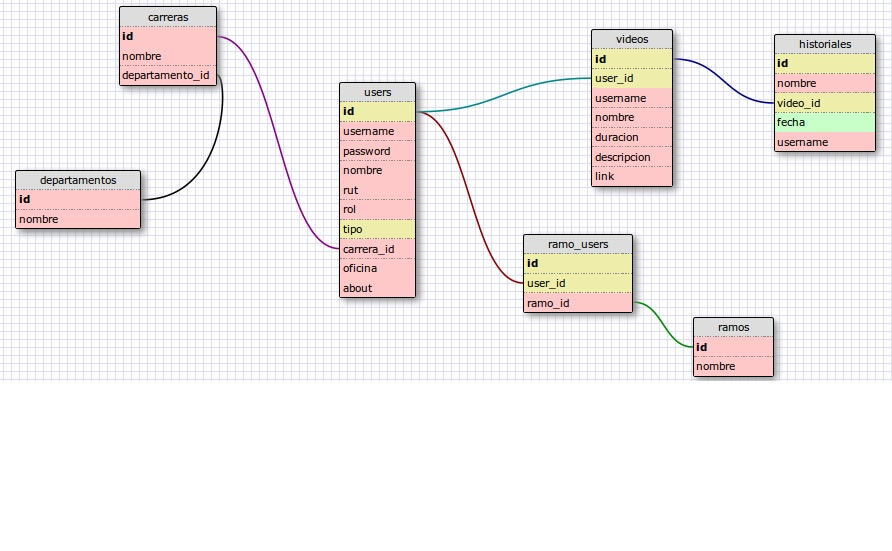
\includegraphics[width=1.0\textwidth]{modelo}
	    \caption{Modelo de Datos}
	\label{fig:moddatos}
\end{figure}


\end{document}

